% This is samplepaper.tex, a sample chapter demonstrating the
% LLNCS macro package for Springer Computer Science proceedings;
% Version 2.21 of 2022/01/12
%
\documentclass[runningheads]{llncs}
%
\usepackage[german]{babel}
\usepackage[T1]{fontenc}
% T1 fonts will be used to generate the final print and online PDFs,
% so please use T1 fonts in your manuscript whenever possible.
% Other font encondings may result in incorrect characters.
%
\usepackage{graphicx}
\usepackage{float}
\usepackage{subcaption}
\usepackage{amsmath}
% Used for displaying a sample figure. If possible, figure files should
% be included in EPS format.
%
% If you use the hyperref package, please uncomment the following two lines
% to display URLs in blue roman font according to Springer's eBook style:
\usepackage{hyperref}
\usepackage{color}
\renewcommand\UrlFont{\color{blue}\rmfamily}
\urlstyle{rm}
%
\begin{document}
%
\title{Contribution Title}
%
%\titlerunning{Abbreviated paper title}
% If the paper title is too long for the running head, you can set
% an abbreviated paper title here
%
\author{Alina Saskia Simon \and
Jannes Bikker \and
Julian Schöpe \and
Malte Elvers \and
Marvin Stier}
%
\authorrunning{Simon, Bikker, Schöpe, Elvers, Stier}
% First names are abbreviated in the running head.
% If there are more than two authors, 'et al.' is used.
%
\institute{Technische Universität Clausthal, Clausthal-Zellerfeld 38678, Deutschland}
%
\maketitle              % typeset the header of the contribution
%
\begin{abstract}
The abstract should briefly summarize the contents of the paper in
150--250 words.

\keywords{First keyword  \and Second keyword \and Another keyword.}
\end{abstract}
%
%
%
\section{Einleitung}
Da der ursprünglich ausgewählte Datensatz sich, nach ersten Experimenten, als unbrauchbar oder zumindest unvorteilhaft für erste Erfahrungen mit künstlicher Intelligenz herausgestellt hat, ist der folgende Bericht in zwei Teile aufgeteilt. Im ersten Teil werden die Ansätze und Erkenntnisse mit erwähntem verworfenen Datensatz erläutert und im zweiten Teil dann die Arbeit mit dem finalen Datensatz (German Traffic Sign Detection Benchmark).

\subsection{Verworfener Datensatz}
Der zuerst ausgewählte Datensatz, Fruit Quality Dataset~\cite{ref_fruit_dataset}, beinhaltet Bilder mit Labeln nach einem Schema, welches typischerweise für YOLO~\cite{ref_yolo} verwendet wird.

\subsubsection{Preprocessing} Ausgehend von stichprobenartiger Begutachtung der ersten Bild-Label-Paare wurde die erste Zahl in der korrespondierenden Label-Datei als Label verwendet. Später stellte sich heraus, dass es durchaus mehrere Label pro Datei gibt, die auch den folgenden Ansatz unwirksam machen. Die Klassenverteilung war relativ ausgeglichen mit einigen Ausreißern, aber durchaus brauchbar.

\subsubsection{Training} Es wurde ein CNN trainiert mit einem Input von Bildern der Größe 128x128 mit 3 Farbkanälen. Als Ausgang für erste Experimente diente dabei eine Pipeline für Bildklassifikation, welche in einer zurückliegenden Vorlesung als Abschlussprojekt geschrieben wurde. Ein Schritt dabei war die Normalisierung der Farbdaten von [0, 255] auf [0, 1]. In einer ersten Iteration wurde diese Normalisierung aber nur vor dem Training und nicht vor dem Testen mit unbekannten Bildern vorgenommen, weshalb die Ausgabe fehlerhaft war.

Nachdem Flüchtigkeitsfehler berichtigt wurden waren die Ergebnisse jedoch eher unzufriedenstellend mit einer Accuracy von etwa 72\% auf den Trainings- und einer Accuracy von etwa 56\% auf den Testdaten. Grund dafür könnten die später als fehlerhaft herausgestellten Labels sein.

\subsubsection{Auswertung} Neben der Accuracy auf Testdaten wurde auch überprüft, wie sich das Modell auf realen Daten, in diesem Fall selbst aufgenommenen Bildern von Früchten, schlägt. Jedoch scheint die Vorhersage eher zufällig zwischen zwei Klassen (Apfel und Banane) zu wählen, welche auch zwei der am häufigsten auftretenden Klassen sind. An dieser Stelle sei gesagt, dass sich das Ergebnis sicherlich noch verbessern ließe, wenn der Prozess und das Modell auf mehrere Klassen pro Bild angepasst werden würden, jedoch wurden weitere Experimente an dieser Stelle abgebrochen, weil sich der Datensatz als teils fehlerhaft herausstellte.

\subsubsection{Fehlerhafter Datensatz} Bei einer späteren stichprobenartigen Kontrolle der Daten stellte sich heraus, dass viele der Labels falsche Daten beinhalten, so wurden Abbildung~\ref{fig1} korrekterweise zwei Instanzen von "good\_pomegrenate" zugeschrieben, jedoch fälschlicherweise ebenfalls eine Instanz von "good\_lime".

\begin{figure}[H]
    \centering
    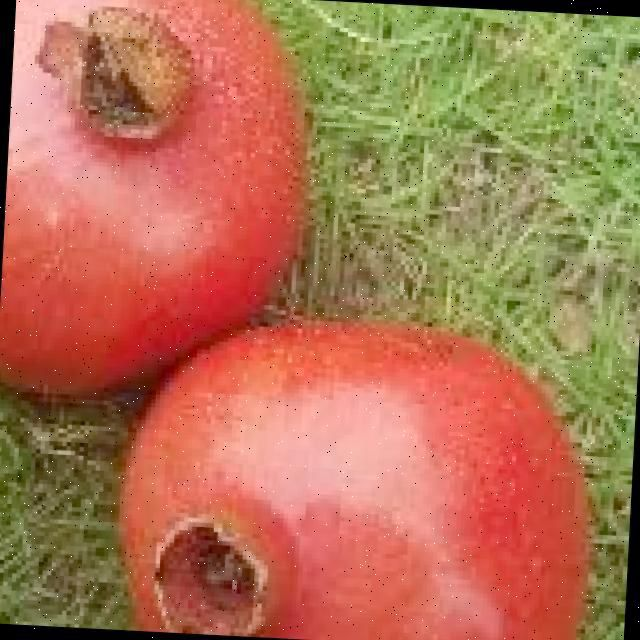
\includegraphics[width=0.5\textwidth]{images/good_pomegrenate_good_lime_error.jpg}
    \caption{Beispielbild aus dem Fruit Quality Dataset mit fehlerhaften Labels.}
    \label{fig1}
\end{figure}

Der grüne Hintergrund lässt demnach auf ungründliches Labeling durch einen Menschen oder möglicherweise bereits eine künstliche Intelligenz schließen. Die Labels konnten demnach nicht für garantiert genommen werden, weshalb ein anderer Datensatz mit sicher korrekten Labels ausgewählt wurde.

\subsubsection{Persönliche Learnings} Datensätze sollten nicht nur für das Verständnis der Form der Daten vor der Verwendung analysiert werden - der Datensatz enthielt pro Bild durchaus mehr als ein Label, wurde aber behandelt als enthielte er nur eins. Sondern es sollte auch die Richtigkeit der Labels und die generelle Qualität der Daten untersucht werden, bevor aufwändiges Training gestartet wird. Zudem sollte vorsichtig mit altem Code umgegangen werden, dessen genaue Funktionalität eventuell schon nicht mehr vollständig bewusst ist, ein möglicher Weg dies zu vermeiden ist die umfassende Dokumentation des Codes.

\section{Zweiter Datensatz: GTSDB}
Der German Traffic Sign Detection Benchmark Datensatz wurde als logische Folgerung aus einer vorherigen Projektarbeit gewählt, in der einige Teammitglieder bereits mit dem German Traffic Sign Recognition Benchmark gearbeitet haben, der Unterschied liegt darin, dass dort bereits auf Schilder ausgeschnittene Bilder für das Training eines CNNs genutzt wurden. Die neue Aufgabe bestand also darin, herauszufinden, wo auf einem Bild Schilder zu erkennen sind, wobei es im ersten Schritt unerheblich ist, um welches Schild es sich genau handelt.

\subsection{Ansätze}
Da ein Modell zur Klassifizierung bereits existierte, wurde ein Ansatz gewählt, in welchem ein entworfenes und trainiertes Modell lediglich Bounding Boxes der Schilder ergeben soll. Dafür würde zum einen HOG (Histogram of Oriented Graphs) mit einer SVM (Support Vector Machine) verwendet werden für einen "klassischeren" Machine Learning Approach mithilfe der "dlib"-Bibliothek. Zum anderen würde auch ein auf Lokalisation ausgerichtetes CNN (Convolutional Neural Network) probiert werden. Die Klassifikation würde in beiden Fällen ein nachgelagertes CNN übernehmen.

\subsection{HOG und SVM}
In diesem ersten Ansatz wird dlib.simple\_object\_detector aus der Bibliothek dlib verwendet, was eine Pipeline für einen Histogram of Oriented Gradients (HOG) basierter Sliding Window Object Detector darstellt~\cite{ref_dlib_docs}, welcher eine Vorhersage mithilfe einer Support Vector Machine (SVM) macht.

\subsubsection{Histogram of Oriented Graphs}
HOG ist eine Art des Preprocessings, beziehungsweise der Featureextraktion. Dabei wird ein Bild mithilfe von zwei Kernels, die ein Bild falten und somit den Informationsgehalt auf Kanten reduzieren können, und dem zusammenfassen in Bins (daher Histogram).

\begin{figure}[H]
    \centering
    \begin{subfigure}{0.45\textwidth}
        \centering
        \[
        H = \begin{pmatrix}
            -1 \\
            0 \\
            1
        \end{pmatrix}
        \]
        \caption{Kernel für horizontale Kanten}
        \label{figKernelsHorizontal}
    \end{subfigure}
    \hfill
    \begin{subfigure}{0.45\textwidth}
        \centering
        \[
        V = \begin{pmatrix}
            -1 & 0 & 1
        \end{pmatrix}
        \]
        \caption{Kernel für vertikale Kanten}
        \label{figKernelsVertical}
    \end{subfigure}
    \caption{Einfache Kernels für die Kantenerkennung}
    \label{figKernels}
\end{figure}

Bei diesen Kernels lässt sich schnell erkennen, dass \ref{figKernelsHorizontal} für einen betrachteten Pixel den darüber negativ und den darunter positiv addiert, wenn also keine Kante sondern eine einfache Farbfläche vorhanden ist, ergibt sich in der Summe 0, beziehungsweise ein kleiner Wert. Wenn aber die Farbwerte stark unterschiedlich ist, ergo an dieser Stelle eine Kante existiert, so ergibt sich ein hoher Wert. Analog dazu ist der Kernel \ref{figKernelsVertical} für vertikale Kanten zuständig.

Zudem werden noch einige Normalisierungen vorgenommen, die hier aber der Einfachheit halber nicht weiter diskutiert werden sollen. In der Abbildung~\ref{fig3} sind das Ursprungsbild und das Ergebnis nach Anwenden der Kernels zu sehen.

\begin{figure}[H]
    \centering
    \begin{subfigure}{0.49\textwidth}
        \centering
        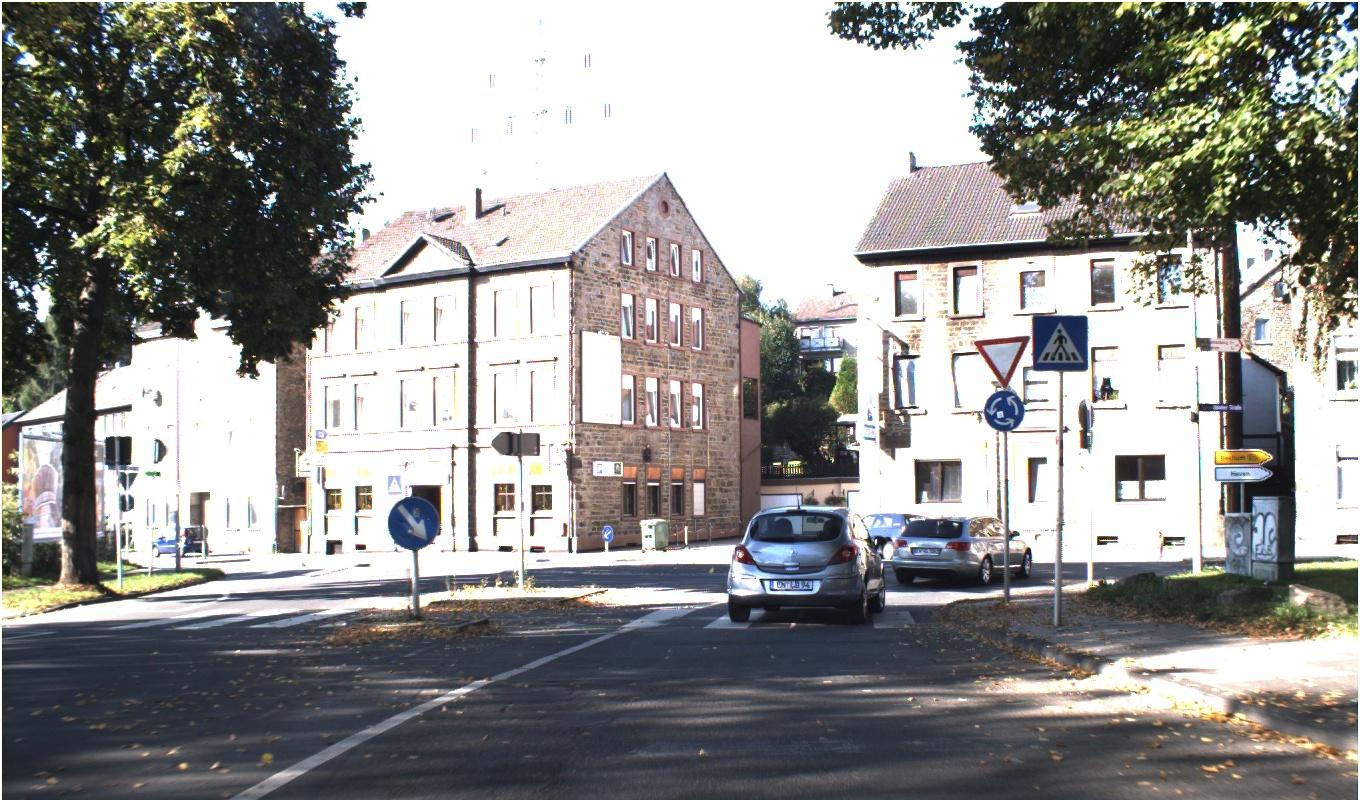
\includegraphics[width=\linewidth]{images/00001.jpg}
        \caption{Ausgangsbild}
        \label{fig3original}
    \end{subfigure}
    \hfill
    \begin{subfigure}{0.49\textwidth}
        \centering
        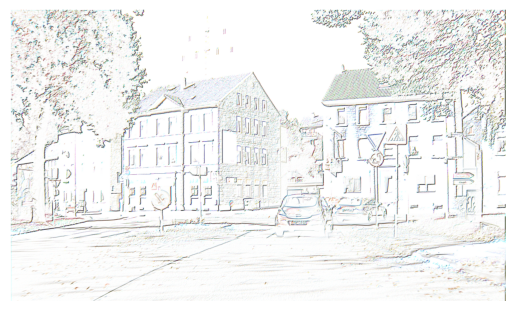
\includegraphics[width=\linewidth]{images/edges_inverted.png}
        \caption{Nach Anwendung der Kernels}
        \label{fig3edges}
    \end{subfigure}
    \caption{Ein Bild vor und nach Anwendung der Kantenkernels (\ref{fig3edges} wurde für bessere Lesbarkeit invertiert).}
    \label{fig3}
\end{figure}

Es ist gut erkennbar, dass der Informationsgehalt auf Kanten reduziert wurde. Für HOG werden die beiden Kernels separat angewendet und jeweils pro Pixel ein Vektor errechnet, der die Kanten beschreibt. Die Längen dieser Vektoren werden in einem Gitternetz über das gesamte Bild in kleineren Gruppen ihrer Richtung nach in Bins aufgeteilt. Danach werden wiederum mehrere beieinanderliegende Gruppen genommen und Stück für Stück normalisiert, um die Werte Resistenter gegen unterschiedliche Beleuchtungen zu machen~\cite{ref_opencv_hog}.

\subsubsection{Support Vector Machine}
Indem ein Erkennungsfenster Stück für Stück über das Bild geschoben wird, welches die minimale Größe der zu erkennenden Objekten festlegt, kann jeweils ein Ausschnitt des berechneten HOG an eine SVM gegeben werden, um zu sagen ob sich dort ein Objekt befindet oder nicht. Diese Art der Objekterkennung eignet sich für unseren Anwendungsfall, weil sämtliche Verkehrschilder auf Formen basieren. In diesem Teilschritt der Verkehrszeichenerkennung wird jedoch nicht zwischen allen verschiedenen Verkehrsschildern unterschieden, sondern sie werden aus genau diesem Grund in formähnliche Gruppen aufgeteilt. Dabei ist nicht die physische Form, sondern die optische Form relevant, ein "Einfahrt verboten" ist zum Beispiel, obwohl es ebenfalls rund ist, in einer anderen Gruppe als "Tempo 30".

\subsubsection{Preprocessing}
Die Bilddaten liegen im .ppm Format vor, welches nicht von gängigen Multimediaprogrammen, sowie der verwendeten Bibliothek erkannt wird. Folglich wurden die Daten ins .jpg Format konvertiert.

In einer ersten Iteration wurden alle Bilder mit zugehörigen Labels in einer von der Bibliothek erkannten XML-Datei gespeichert. Nach späteren Erkenntnissen war es zudem sinnvoll, nach ähnlichen Schilderformen zu gruppieren, zum Beispiel ein Dreieck mit Spitze nach oben, Raute oder Kreis. Für jede dieser Dateien wurde zudem nur ein Teil der Daten ausgewhählt, um neben einer Datei für das Training auch eine Datei für Tests zu generieren.
Eine maßgebliche Limitierung des HOG+SVM Ansatzes ist zudem die Mindestgröße von Objekten. Je nach der Anzahl von Verdopplungen der Bildgröße durch Upsampling variiert diese Größe und gültige Boxen müssen dementsprechend aus den Labels gefiltert werden.

\subsubsection{Training}
Im ersten Durchlauf des Trainings wurden zufällige 80\% aller Bilder des Datensatzes benutzt. Das Ergebnis lies sich sehen mit einer Precision von etwa 87\%. Jedoch fiel die Performance bei weniger stark im Datensatz vertretenen Klassen deutlich schlechter mit bis zu 0\% Precision aus.

In einem nächsten Durchlauf wurden die nach Formen getrennten Trainigs- und Testdateien verwendet und deutlich bessere Ergebnisse in den meisten Kategorien erzielt. In Kategorien mit sehr wenig Trainigsdaten blieb die Precision jedoch bei 0\%, da insgesamt aber nur zwei oder 14 passende Bilder für das Training (und dementsprechend noch weniger für Tests) verfügbar sind, sind diese Ergebnisse nicht vollständig unerwartet.

Um die Erkennung von kleineren Objekten zu verbssern, kann das Bild hochskaliert werden, jedoch stark auf Kosten des verwendeten Arbeitsspeichers. Die verwendete Bibliothek ist auf eine Weise implementiert, sodass der gesamte Trainingsdatensatz vollständig in den Arbeitsspeicher geladen und hochskaliert wird. Verwendete Hardware limitierte daher auf maximal einfache Verdopplung der Auflösung.

\subsubsection{Validierung und Limitierungen}
Um die Ergebnisse manuell auf Anwendbarkeit zu überprüfen wurde eine einfache Anwendung entworfen, welche zufällige Bilder des Datensatzes lädt und alle verfügbaren Modelle anwendet. Ergebnisse mit einer Confidence über einem gestzten Threshold werden dann mit einer Box und dem zugehörigen Label angezeigt, wie in Abbildung~\ref{fig2} zu sehen.

\begin{figure}[H]
    \centering
    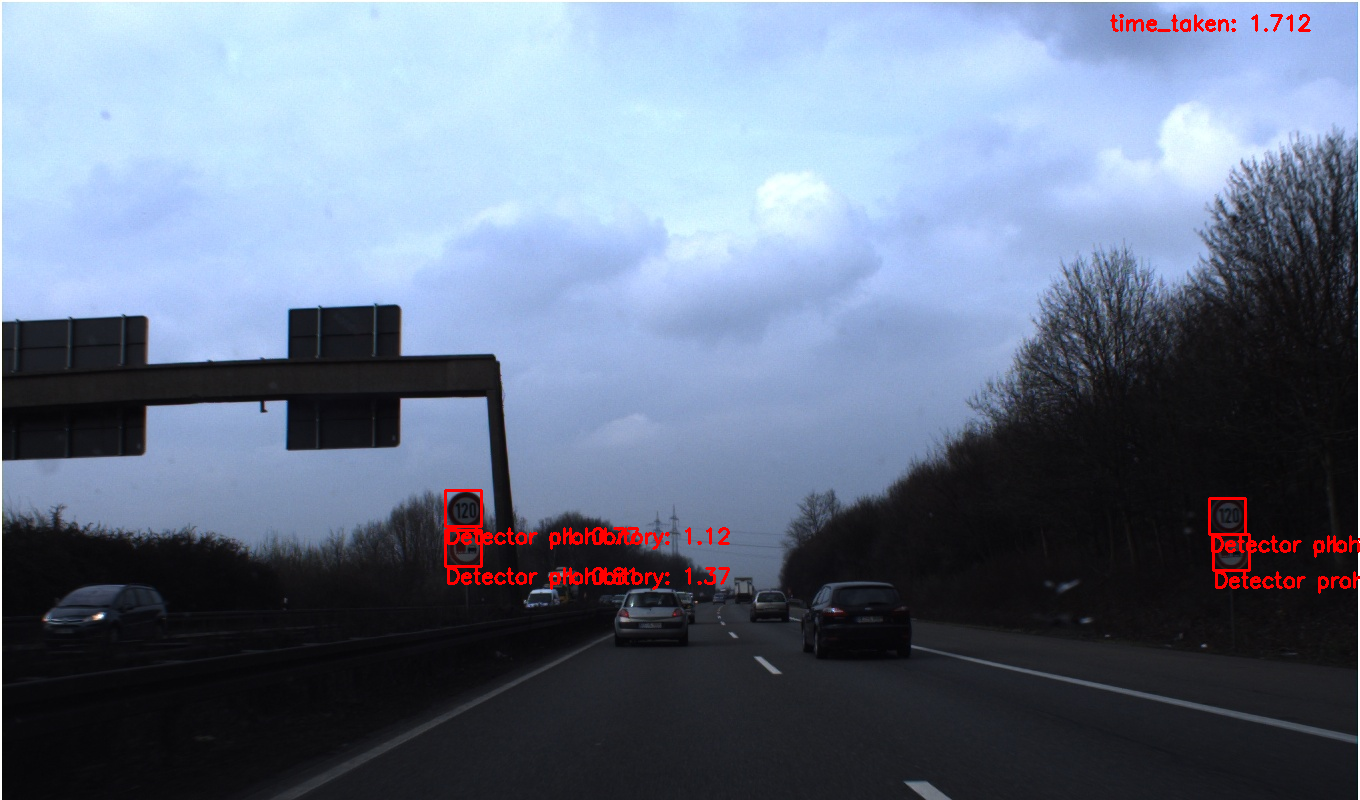
\includegraphics[width=1\textwidth]{images/example_prediction.png}
    \caption{Verkehrsschildlokalisation mit HOG und SVM.}
    \label{fig2}
\end{figure}

Die größte Einschränkung dieses Ansatzes ist die Geschwindigkeit des Modells. Auf durchschnittlicher Laptop-Hardware dauert eine Ausführung etwa 1,7 Sekunden - im Kontext Verkehrsschilderkennung insbesondere auf der Autobahn wäre dies kein akzeptabler Wert. Zudem haben die Modelle mit kleinen Objekten Probleme, da die Erkennungsfenster eine minimale Größe haben.

\section{Lokalisierung mittels Convolutional Neural Network (CNN)}

\subsection{Bounding-Box-Regression}
Als weiterer Ansatz für die Lokalisierung der Verkehrsschilder sollte ein CNN verwendet
werden, um sämtliche Schilder effizient aus einem Bild zu extrahieren.
Der erste Versuch setzte auf eine einfache Bounding-Box-Regression, bei der das Modell
direkt die Koordinaten der Box vorhergesagt hat. Allerdings lernte das Netz dabei, die
Box immer in die Bildmitte zu setzen, da es keine explizite Methode zur Lokalisierung hatte. Statt tatsächlich Schilder zu finden, minimierte es den durchschnittlichen Fehler, was dazu führte, dass es eine zentrale Position bevorzugte.
\\
Dieser Effekt tritt auf, weil das Modell versucht, die Fehler über alle Trainingsbilder
hinweg zu minimieren. Wenn sich Schilder an vielen verschiedenen Positionen befinden,
aber keine klare Methode zur Bestimmung der genauen Position existiert, wählt das
Modell eine Durchschnittsposition für seine Vorhersagen. Die Bildmitte ist oft die
statistisch sicherste Wahl, weil sie den kleinsten mittleren Fehler zu allen tatsächlichen
Positionen liefert und das Modell mit dem Wert des mittleren Fehlers bestimmt wie "gut"
eine Vorhersage im Training ist. Anstatt dynamisch die richtige Position für jedes Bild
zu berechnen,
erkennt das Modell fälschlicherweise ein Muster:
Es kann den Fehler über viele Bilder hinweg reduzieren, indem es einfach immer eine
Box mittig platziert, da das Training darauf abzielt, die durchschnittliche
Abweichung zu minimieren. Ohne eine Möglichkeit, lokale Merkmale effektiv mit einer
bestimmten Position zu verknüpfen, bleibt das Modell
in diesem Muster gefangen.

\subsection{Weiterer Ansatz}

Um dieses Problem zu lösen, wurde ein Modell basierend auf einem Faster R-CNN eingesetzt.
Dieses Modell kombiniert ein klassisches CNN mit einem Mechanismus zur Objekterkennung.
Anstatt direkt eine Bounding Box vorherzusagen, sucht es zunächst nach wahrscheinlichen
Objektregionen und bewertet, ob dort ein Verkehrsschild vorhanden ist.
Dies ermöglicht eine dynamische und adaptive Erkennung, anstatt starr eine feste Position
zu wählen.
\\
Ein wichtiger Bestandteil dieses Modells ist das Backbone, ein CNN, in unserem Fall
ResNet-50, das als Feature-Extractor dient. Das Backbone verarbeitet das Bild und extrahiert
wichtige Merkmale, wie Kanten und Formen, die für die Objekterkennung relevant sind.
Diese abstrahierten Informationen helfen dem nachfolgenden Region Proposal Network (RPN),
gezielt Bereiche zu identifizieren, in denen sich wahrscheinlich Schilder befinden.
\\
Um diesen Ansatz umzusetzen, wurde ein Trainingsmodell mit PyTorch erstellt.
Zunächst wurde ein Datensatzloader erstellt, der die Trainingsbilder aus einem Ordner lädt
und die zugehörigen Bounding-Box-Koordinaten aus der Annotationsdatei einliest.
Das Modell benötigt standardisierte Eingaben, daher werden alle Bilder auf eine feste
Größe skaliert und die Bounding-Box-Koordinaten ebenfalls entsprechend angepasst.
\\
Für das Modell selbst wurde ein Faster R-CNN mit ResNet-50 als Backbone genutzt und dessen
Head angepasst, um die Erkennung von Verkehrsschildern als einzig relevante Klasse zu
ermöglichen. Das Modell klassifiziert nur in zwei Klassen: Hintergrund und Verkehrsschild.
Das Training wurde mit einer Stochastic Gradient Descent (SGD)-Optimierung durchgeführt,
wodurch die Modellparameter iterativ basierend auf den Gradienten der Verlustfunktion
angepasst werden. Dabei kam Mixed Precision Training zum Einsatz, um GPU-Berechnungen
effizienter zu gestalten und Speicher zu sparen. Dies passiert durch den Einsatz von
16-bit und 32-bit-Floating-Point-Werten, wobei kritische Berechnungen in höherer
Genauigkeit durchgeführt werden\cite{ref_mixed_precision_nvidia}.
Das Training wurde über mehrere Epochen hinweg durchgeführt, wobei das Modell die Fehler
reduzierte und bessere Vorhersagen lieferte. Mit 10 Epochen konnte das Modell schon
zuverlässig Verkehrsschilder lokalisieren, 20 Epochen haben die Genauigkeit allerdings nur
marginal verbessert.
\\
Nach Abschluss des Trainings wurde das trainierte Modell gespeichert und kann verwendet
werden, um mehrere Verkehrsschilder in einem Bild zu erkennen. Das Modell gibt für jedes
gefundene Schild eine Bounding Box mit einer Wahrscheinlichkeit aus.

\section{Recognition mittels Convolutional Neural Network (CNN)}
Zur Erkennung der Bildklassen/Straßenschilder wurde ein Convolutional Neural Network (CNN) implementiert. Die Architektur des Modells wurde
durch eine Kombination aus grundlegendem theoretischem Verständnis der einzelnen Schichten und Trial-and-Error entwickelt.
Während grundlegende Konzepte wie Faltungsschichten (Convolutional Layers), Aktivierungsfunktionen und Batch-Normalisierung
bekannt waren, wurde die genaue Anordnung und Anzahl der Schichten durch einfaches Testen bestimmt.
Zum trainieren, validieren und teste des Modells wurde der German Traffic Sign Recognition Benchmark (GTSRB) Datensatz genutzt, der
im Vergleich zum GTSDB Datensatz schon lokalisierte Schilder enthält.

\subsection{Modellarchitektur}
Die Modellarchitektur wurde durch einen stumpfen Trial-and-Error Prozess entwickelt. Zwar bestand ein grundlegendes Verständnis
für die einzelnen Schichten und ihre Funktion, jedoch wurde die endgültige Struktur experimentell bestimmt.
Erst nachdem ein gut funktionierendes Modell gefunden war, wurde die genaue Zusammenarbeit der Schichten angeschaut und
nachvollzogen. Das finale Modell besteht aus mehreren Convolutional Layers (Conv2D) mit ReLU-Aktivierung und Kernel-Regularisierung
zur Merkmalsextraktion. Batch-Normalisierung stabilisiert den Trainingsprozess, während Max-Pooling-Schichten die räumlichen
Dimensionen reduzieren und Overfitting entgegenwirken. Zusätzlich sorgen Dropout-Schichten für eine bessere Generalisierung.
Abschließend übernimmt eine vollständig verbundene (Dense) Schicht mit Softmax-Aktivierung die Klassifikation der Eingabedaten.

\subsection{Training des Modells}
Die Trainingsbilder wurden zufällig um einen Winkel zwischen -10 und +10 Grad rotiert (layers.RandomRotation(0.1)). Dies soll das Modell
robuster gegen leichte Drehungen und Orientationsänderungen der Verkehrsschilder machen, die in realen Szenarien auftreten können. Ein Beispiel
hierfür ist in \ref{fig4} zu sehen. Das Modell wurde mit der Adam-Optimierungsmethode trainiert, wobei eine Lernrate von $0.001$ verwendet wurde. Zudem wurde ein
Learning Rate Scheduler eingesetzt (ReduceLROnPlateau), um die Lernrate bei Stagnation automatisch zu reduzieren.

\begin{figure}[H]
    \centering
    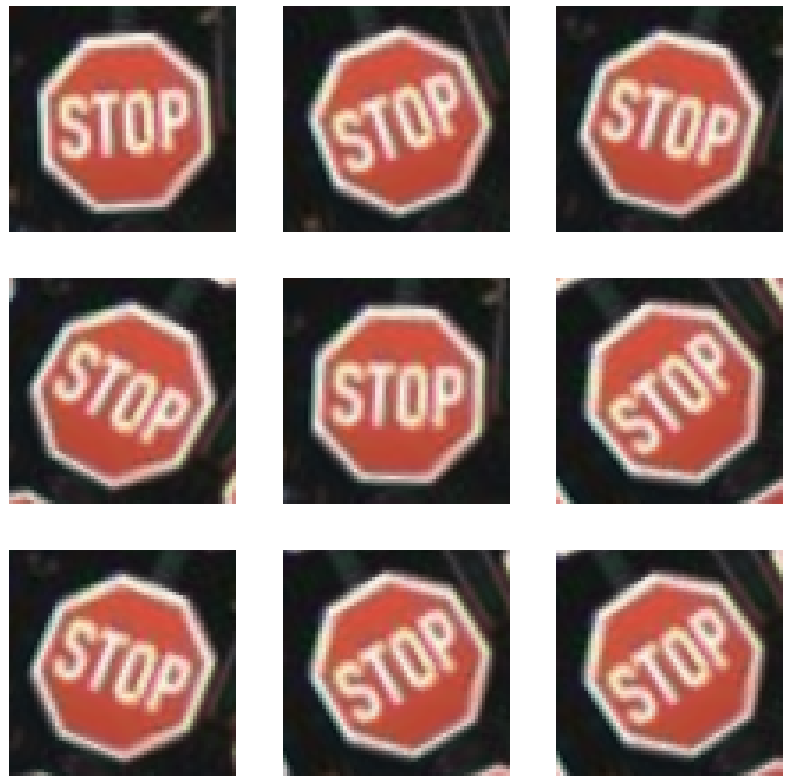
\includegraphics[width=0.5\textwidth]{images/RandomRotation.png}
    \caption{Beispiel für zufällige Rotation der Trainingsdaten.}
    \label{fig4}
\end{figure}

Die Loss-Funktion ist die kategoriale Kreuzentropie, da es sich um ein Mehrklassen-Klassifikationsproblem handelt.
Um Overfitting zu vermeiden, wurden Early Stopping und Model Checkpoints verwendet. Diese hatten außerdem den Vorteil, dass
das bei Bedarf bestimmte Versionen des Modells gespeichert und im Nachhinein genutzt wurden konnten.

\subsection{Modellbewertung}
Das Modell wurde nach dem Training mit einem separaten Testdatensatz evaluiert. Dabei wurden die Genauigkeit sowie die mittlere
Konfidenz der Vorhersagen betrachtet. Fehlklassifizierungen wurden ausgegeben, um mögliche Schwachstellen zu identifizieren.
Neben der Gesamtperformance des Modells wurde jede Schildklasse einzeln betrachtet, um die Performance des Modells für jede Klasse bewerten zu können.

Durch die Schildklassen betrachtung zeigte sich, dass insbesondere die Kategorie der Verbotszeichen mit der markanten roten
Diagonalen eine Herausforderung für das Modell darstellten. Diese Schwierigkeit ist vermutlich darauf zurückzuführen, dass die Diagonale
zwar ein starkes Unterscheidungsmerkmal darstellt, jedoch bei vielen verschiedenen Verbotszeichen vorhanden ist.

\subsection{Nutzung des trainierten Modells}

Das trainierte Modell wurde im .h5-Format gespeichert, einem von Keras verwendeten Format, das die Serialisierung der
Modellarchitektur und der Gewichte ermöglicht. Konkret bedeutet dies, dass das .h5-File mittels tf.keras.models.load\_model()
geladen werden kann. Anschließend können Verkehrsschildbilder dem Modell zur Klassifizierung übergeben werden und das Modell
gibt die vorhergesagte Klasse zurück.

\subsection{Teil Fazit CNN}
Die Entwicklung der CNN-Architektur folgte keinem strikt vorgegebenen Schema, sondern entstand durch schrittweises Experimentieren.
Durch Anpassungen und Tests wurde eine Modellstruktur gefunden, die das gewünschte Ergebnis liefert. Die Klassifizierung des
Finalen Modells war sowohl auf dem Testdatensatz als auch auf dem Output des Lokalisierungsmodells sehr gut.


%\paragraph{Sample Heading (Fourth Level)}
%The contribution should contain no more than four levels of
%headings. Table~\ref{tab1} gives a summary of all heading levels.

% \begin{table}
% \caption{Table captions should be placed above the
% tables.}\label{tab1}
% \begin{tabular}{|l|l|l|}
% \hline
% Heading level &  Example & Font size and style\\
% \hline
% Title (centered) &  {\Large\bfseries Lecture Notes} & 14 point, bold\\
% 1st-level heading &  {\large\bfseries 1 Introduction} & 12 point, bold\\
% 2nd-level heading & {\bfseries 2.1 Printing Area} & 10 point, bold\\
% 3rd-level heading & {\bfseries Run-in Heading in Bold.} Text follows & 10 point, bold\\
% 4th-level heading & {\itshape Lowest Level Heading.} Text follows & 10 point, italic\\
% \hline
% \end{tabular}
% \end{table}


% \noindent Displayed equations are centered and set on a separate
% line.
% \begin{equation}
% x + y = z
% \end{equation}
% Please try to avoid rasterized images for line-art diagrams and
% schemas. Whenever possible, use vector graphics instead (see
% Fig.~\ref{fig1}).

% \begin{theorem}
% This is a sample theorem. The run-in heading is set in bold, while
% the following text appears in italics. Definitions, lemmas,
% propositions, and corollaries are styled the same way.
% \end{theorem}
%
% the environments 'definition', 'lemma', 'proposition', 'corollary',
% 'remark', and 'example' are defined in the LLNCS documentclass as well.
%
% \begin{proof}
% Proofs, examples, and remarks have the initial word in italics,
% while the following text appears in normal font.
% \end{proof}
% For citations of references, we prefer the use of square brackets
% and consecutive numbers. Citations using labels or the author/year
% convention are also acceptable. The following bibliography provides
% a sample reference list with entries for journal
% articles~\cite{ref_article1}, an LNCS chapter~\cite{ref_lncs1}, a
% book~\cite{ref_book1}, proceedings without editors~\cite{ref_proc1},
% and a homepage~\cite{ref_url1}. Multiple citations are grouped
% \cite{ref_article1,ref_lncs1,ref_book1},
% \cite{ref_article1,ref_book1,ref_proc1,ref_url1}.

% \begin{credits}
% \subsubsection{\ackname} A bold run-in heading in small font size at the end of the paper is
% used for general acknowledgments, for example: This study was funded
% by X (grant number Y).

% \subsubsection{\discintname}
% It is now necessary to declare any competing interests or to specifically
% state that the authors have no competing interests. Please place the
% statement with a bold run-in heading in small font size beneath the
% (optional) acknowledgments\footnote{If EquinOCS, our proceedings submission
% system, is used, then the disclaimer can be provided directly in the system.},
% for example: The authors have no competing interests to declare that are
% relevant to the content of this article. Or: Author A has received research
% grants from Company W. Author B has received a speaker honorarium from
% Company X and owns stock in Company Y. Author C is a member of committee Z.
% \end{credits}
%
% ---- Bibliography ----
%
% BibTeX users should specify bibliography style 'splncs04'.
% References will then be sorted and formatted in the correct style.
%
% \bibliographystyle{splncs04}
% \bibliography{mybibliography}
%
\begin{thebibliography}{8}
\bibitem{ref_dlib_docs}
dlib Python Dokumentation, \url{https://dlib.net/python/index.html}, letzter Zugriff 16.02.2025

\bibitem{ref_fruit_dataset}
Fruit Quality Dataset auf Kaggle, \url{https://www.kaggle.com/datasets/abrars2/fruit-quality-classificaltion-and-detection}, letzter Zugriff 15.02.2025

\bibitem{ref_opencv_hog}
Histogram of Oriented Gradients explained using OpenCV, \url{https://learnopencv.com/histogram-of-oriented-gradients/}, letzter Zugriff 16.02.2025

\bibitem{ref_medium_hog}
A Gentle Introduction Into The Histogram Of Oriented Graphs, \url{https://medium.com/analytics-vidhya/a-gentle-introduction-into-the-histogram-of-oriented-gradients-fdee9ed8f2aa}, letzter Zugriff 16.02.2025

\bibitem{ref_grundlagenki_folien}
Marton, S.: Grundlagen der KI Foliensatz (2025)

\bibitem{ref_yolo}
YOLO Framework, \url{https://zenodo.org/records/7347926}, letzter Zugriff 15.02.2025

\bibitem{ref_mixed_precision_nvidia}
Mixed Precision Training, \url{https://docs.nvidia.com/deeplearning/performance/mixed-precision-training/index.html}, letzter Zugriff 16.02.2025

% \bibitem{ref_lncs1}
% Author, F., Author, S.: Title of a proceedings paper. In: Editor,
% F., Editor, S. (eds.) CONFERENCE 2016, LNCS, vol. 9999, pp. 1--13.
% Springer, Heidelberg (2016). \doi{10.10007/1234567890}

% \bibitem{ref_book1}
% Author, F., Author, S., Author, T.: Book title. 2nd edn. Publisher,
% Location (1999)

% \bibitem{ref_proc1}
% Author, A.-B.: Contribution title. In: 9th International Proceedings
% on Proceedings, pp. 1--2. Publisher, Location (2010)

% \bibitem{ref_url1}
% LNCS Homepage, \url{http://www.springer.com/lncs}, last accessed 2023/10/25
\end{thebibliography}
\end{document}
